\iffalse
\documentclass[10pt]{article}
\usepackage{graphicx}
\def\inputGnumericTable{}
\usepackage[latin1]{inputenc}
\usepackage{fullpage}
\usepackage{color}
\usepackage{array}
\usepackage{longtable}
\usepackage{calc}
\usepackage{multirow}
\usepackage{hhline}
\usepackage{ifthen}
\usepackage{amsmath}
\usepackage[none]{hyphenat}
\usepackage{listings}
\usepackage[english]{babel}
\usepackage{siunitx}
\usepackage{caption}
\usepackage{booktabs}
\usepackage{array}
\usepackage{extarrows}
\usepackage{enumerate}
\usepackage{enumitem}
\usepackage{amsmath}
\usepackage{commath}
\usepackage{gensymb}
\usepackage{amssymb}
\usepackage{multicol}
%\usepackage[utf8]{inputenc}
\lstset{
 frame=single,
 breaklines=true
}
\usepackage{hyperref}
\usepackage[margin=0.65in]{geometry}	 
%\usepackage{exsheets}% also loads the `tasks' package
\usepackage{atbegshi}
\AtBeginDocument{\AtBeginShipoutNext{\AtBeginShipoutDiscard}}

%new macro definitions
\renewcommand{\labelenumi}{(\roman{enumi})}
\newcommand{\mydet}[1]{\ensuremath{\begin{vmatrix}#1\end{vmatrix}}}
\providecommand{\brak}[1]{\ensuremath{\left(#1\right)}}
\newcommand{\solution}{\noindent \textbf{Solution: }}
\newcommand{\myvec}[1]{\ensuremath{\begin{pmatrix}#1\end{pmatrix}}}
\newenvironment{amatrix}[1]{%
	\left(\begin{array}{@{}*{#1}{c}|c@{}}
}{%
	\end{array}\right)
}

\newcommand{\myaugvec}[2]{\ensuremath{\begin{amatrix}{#1}#2\end{amatrix}}}
\providecommand{\norm}[1]{\left\1Vert#1\right\rVert}
\let\vec\mathbf{}


%\SetEnumitemKey{twocol}{
% before=\raggedcolumns\begin{multicols}{2},
% after=\end{multicols}}
%\SetEnumitemKey{fourcol}{
% before=\raggedcolumns\begin{multicols}{4},
% after=\end{multicols}} 


\begin{document}
\begin{center}
\title{\textbf{TRIANGLES}}
\date{\vspace{-5ex}}
\maketitle
\end{center}
\section*{9$^{th}$Math - Chapter 7}
This is Problem-8 from Exercise 7.1\\\\


\section*{\large Construction:}
\fi
The input parameters for construction
	are available in Table \ref{tab:chapters/9/7/1/8/table}.
\begin{table}[h!]
	\centering
	%\subimport{../chapters/9/7/1/8/tables/}{table.tex}
     \begin{tabular}{|c|c|p{5cm}|}
\hline
\textbf{Symbol} & \textbf{Value} & \textbf{Description} \\
\hline
$\theta$ & $30\degree$ & $\angle{BAP} = \angle{BAQ}$ \\
\hline
$a$ & $9$ & $AB$ \\
\hline
$c$ & $8$ & $AQ$ \\
\hline
$\vec{e}_1$ & $\myvec{1\\0}$ & Basis vector \\
\hline
\end{tabular}

	\caption{}
	\label{tab:chapters/9/7/1/8/table}
\end{table}
Thus, 
\begin{align}
	\vec{A}=\myvec{0\\b},\,
	\vec{B}=\myvec{a\\0},\,
	\vec{C}=\myvec{0\\0}
\end{align}
yielding
\begin{align}
	\vec{M}&=\frac{\vec{A}+\vec{B}}{2}=\frac{1}{2}\myvec{a\\b}
\end{align}
Also, 
\begin{align}
	\vec{M}&=\frac{\vec{C}+\vec{D}}{2}\\
	\implies \vec{D}&=2\vec{M}-\vec{C}=\myvec{a\\b}
\end{align}
\iffalse
\solution
Given
\begin{align}
	\vec{M}&=\frac{\vec{A}+\vec{B}}{2}
	\label{eq:chapters/9/7/1/8/1}\\
	\vec{D}-\vec{M}&=\vec{C}-\vec{M}
	\label{eq:chapters/9/7/1/8/2}\\
	\angle ACB&=90\degree
\end{align}
\textbf{Proof:} From Figure \ref{fig:chapters/9/7/1/8/1}
\fi
Thus,
\begin{align}
	\brak{\vec{D}-\vec{B}}^{\top}\brak{\vec{B}-\vec{C}} &= \myvec{0 & b}\myvec{a\\0}=0\\
	\implies BD & \perp BC\\
\end{align}
Also, 
\begin{align}
	\norm{\vec{A}-\vec{B}}&=\norm{\myvec{-a\\b}}\\
	\norm{\vec{C}-\vec{D}}&=\norm{\myvec{-a\\-b}}\\
	\implies \norm{\vec{A}-\vec{B}} &= \norm{\vec{C}-\vec{D}}\\
	\text{ or, } AB &= CD
	\label{eq:chapters/9/7/1/8/3}	
\end{align}
From \eqref{eq:chapters/9/7/1/8/3}
\begin{align}
	\implies CM = \frac{1}{2}CD = \frac{1}{2}AB 
\end{align}
See Fig. 
\ref{fig:chapters/9/7/1/8/1}.
\begin{figure}[H]
	\begin{center}
		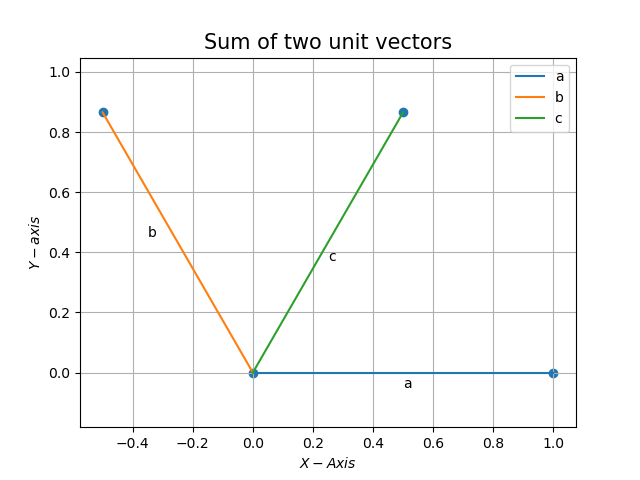
\includegraphics[width=\columnwidth]{./chapters/9/7/1/8/figs/fig.pdf}
	\end{center}
\caption{}
\label{fig:chapters/9/7/1/8/1}
\end{figure}

